\documentclass[a4paper,14pt]{extarticle}
\usepackage{graphicx}
\usepackage{amsmath}
\usepackage{geometry}
\usepackage{float}

\geometry{margin=1in}

\title{Online Book Store Management System}
\author{}
\date{}

\begin{document}

\maketitle

\section*{\centering Team Members}
\begin{center}
    \begin{tabular}{c}
        Adam Tamer \\
        Mohamed Tarek \\
        Sara Mahmoud
    \end{tabular}
\end{center}

\section*{UML Diagram}

\begin{figure}[H]
    \centering
    \makebox[\textwidth][c]{%
        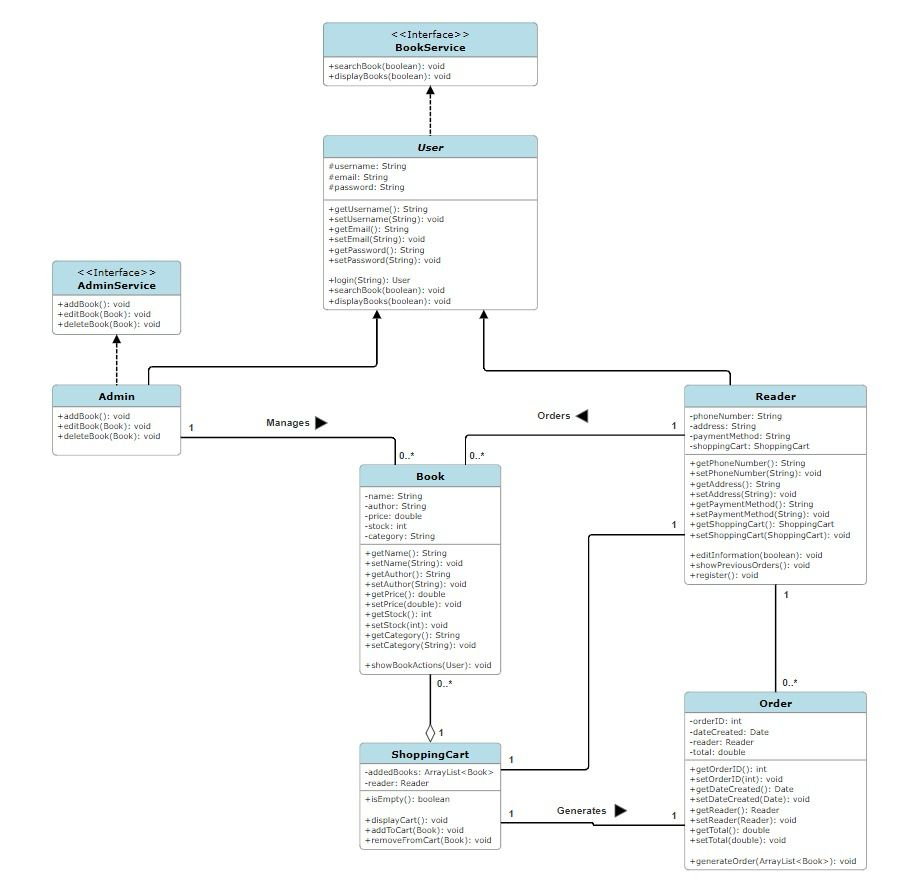
\includegraphics[width=1.2\textwidth]{Media/UML.jpeg}
    }
    \caption{UML Diagram}
\end{figure}


\newpage
\section*{Overview of the System}
\begin{figure}[H]
    \centering
    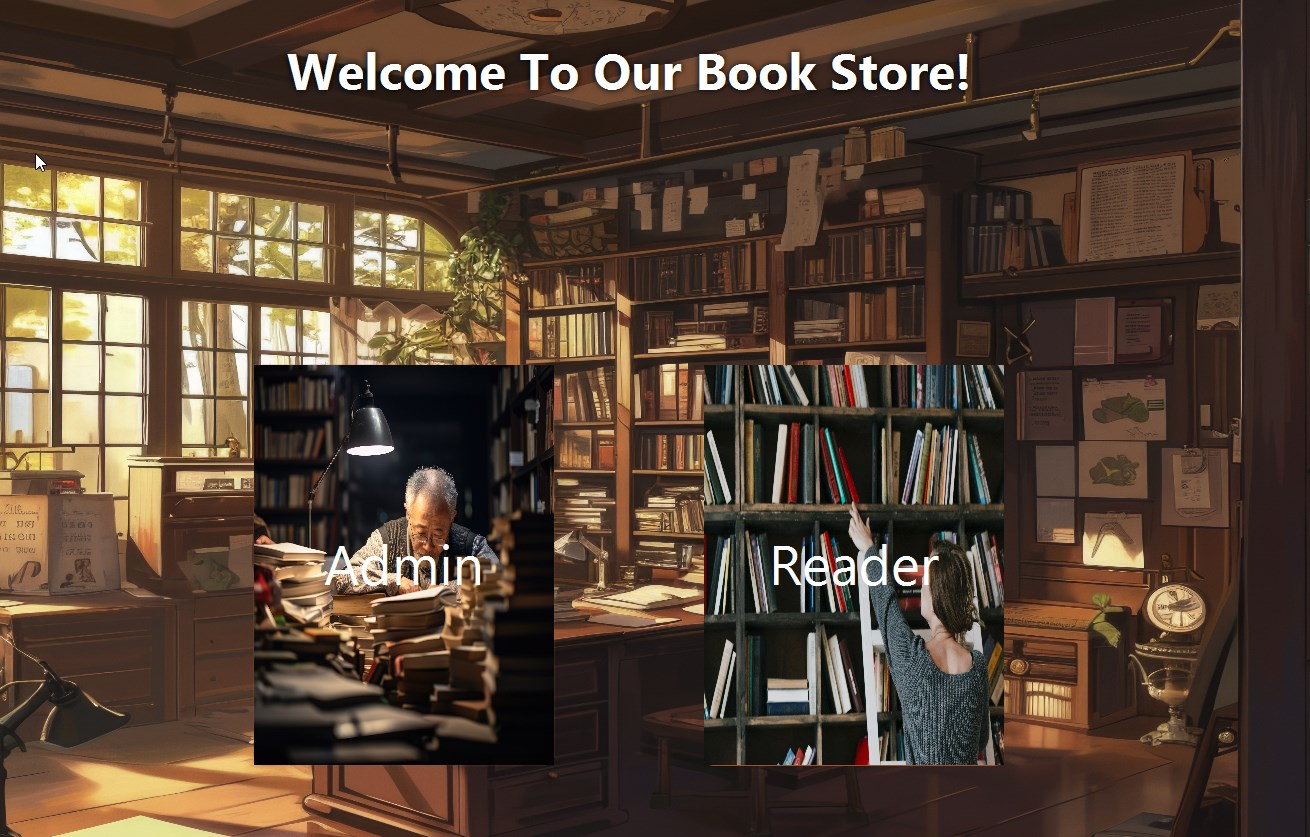
\includegraphics[width=0.8\textwidth]{Media/Main Page.jpg}
    \caption{Main Menu}
\end{figure}

\begin{figure}[H]
    \centering
    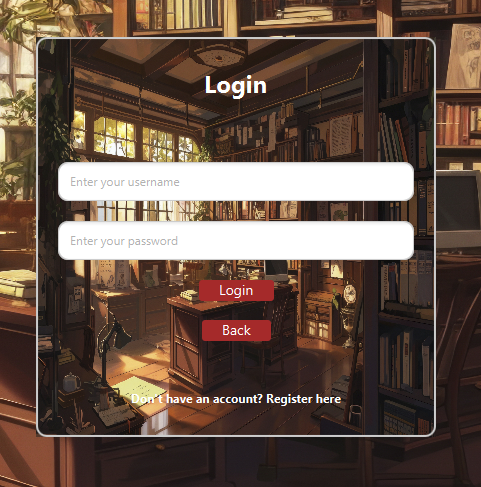
\includegraphics[width=0.6\textwidth]{Media/Login.png}
    \caption{Login Page}
\end{figure}
\newpage
\section*{Admin Functions}

\begin{figure}[H]
    \centering
    \makebox[\textwidth][c]{%
        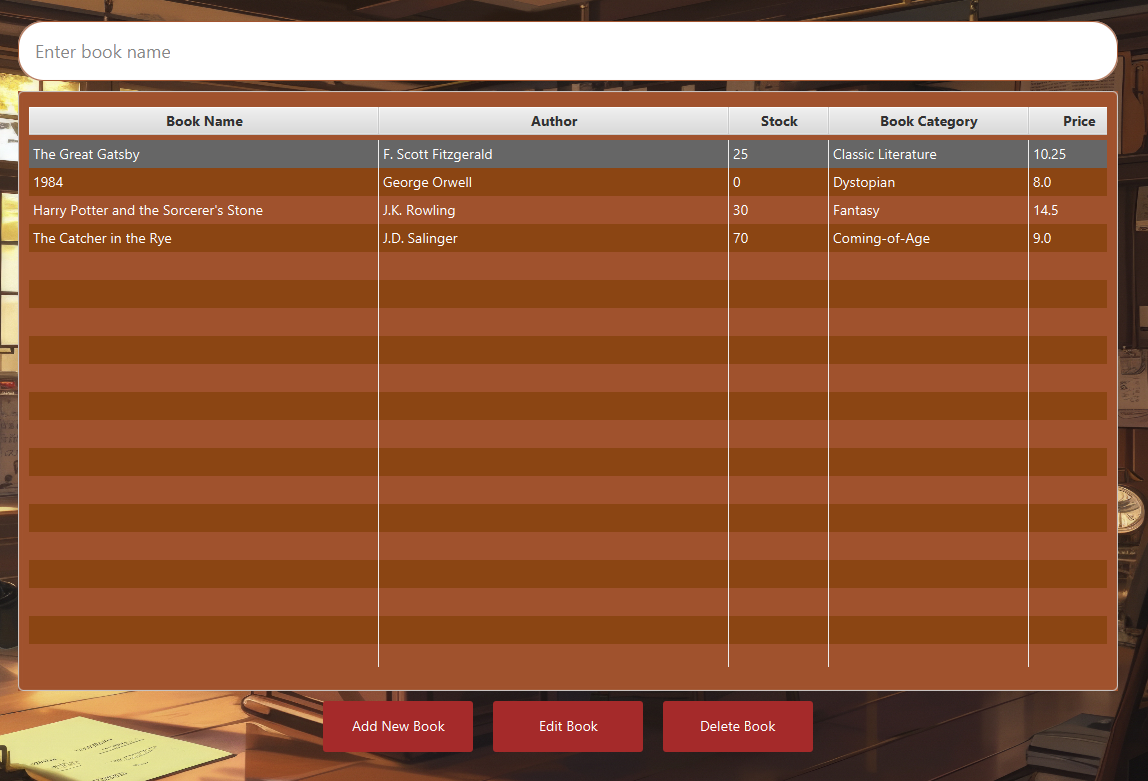
\includegraphics[width=\textwidth]{Media/admin.png}
    }
    \caption{Admin Menu}
\end{figure}


\begin{figure}[H]
    \centering
    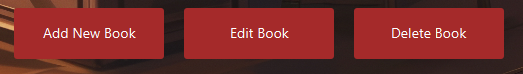
\includegraphics[width=0.85\textwidth]{Media/Admin Functions.png}
    \caption{Admin Functions Overview}
\end{figure}
\newpage
\begin{itemize}
    \item \textbf{Add a Book:} The admin can add new books to the store's inventory using the "Add New Book" dialog. Once the admin fills in the book's data, pressing save will call the 
    \texttt{add\-Book(Book book)} method.
    \begin{figure}[H]
        \centering
        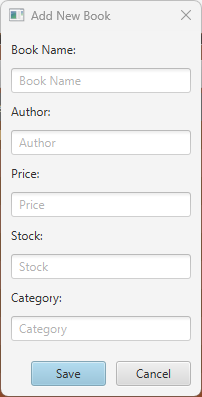
\includegraphics[width=0.4\textwidth]{Media/Add New Book.png}
        \caption{Add New Book Dialog}
    \end{figure}
    \begin{figure}[H]
        \centering
        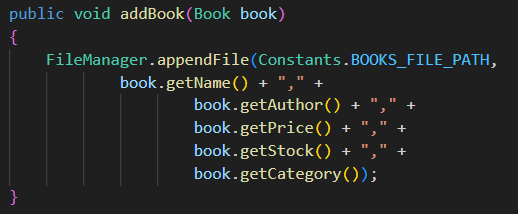
\includegraphics[width=0.75\textwidth]{Media/addBook.png}
        \caption{addBook Implementation}
    \end{figure}
\newpage
    \item \textbf{Edit a Book:} The admin can edit the details of an existing book using the "Edit Book" dialog. Once the admin modifies the book's data, pressing save will call the 
    \texttt{edit\-Book(Book book, Book updated\-Book)} method.
    \begin{figure}[H]
        \centering
        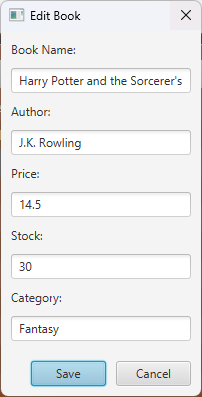
\includegraphics[width=0.35\textwidth]{Media/Edit Book.png}
        \caption{Edit Book Dialog}
    \end{figure}

    \begin{figure}[H]
    \centering
    \makebox[\textwidth][c]{%
        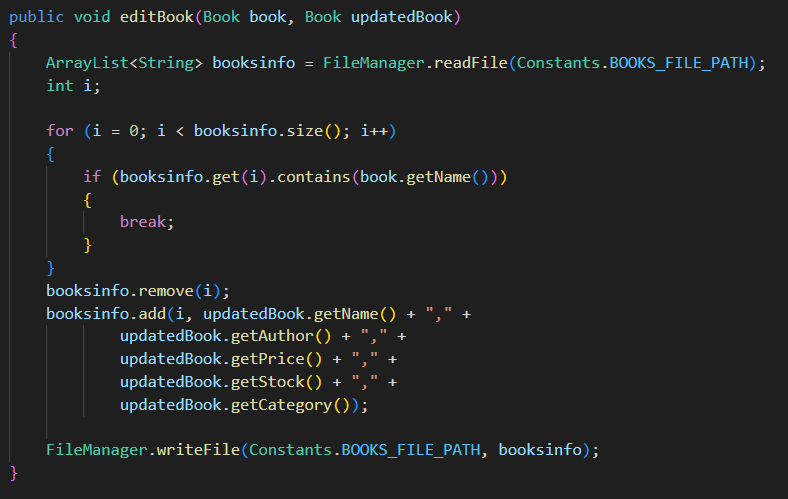
\includegraphics[width=0.8\textwidth]{Media/editBook.png}
    }
        \caption{editBook Implementation}
\end{figure}

    \item \textbf{Delete a Book:} The admin can remove a book from the store's inventory using the \texttt{delete\-Book(Book book)} method.
    \begin{figure}[H]
        \centering
        
\includegraphics[width=0.35\textwidth]{Media/Delete Book.png}
        \caption{Delete Book Button}
    \end{figure}
    \begin{figure}[H]
        \centering
        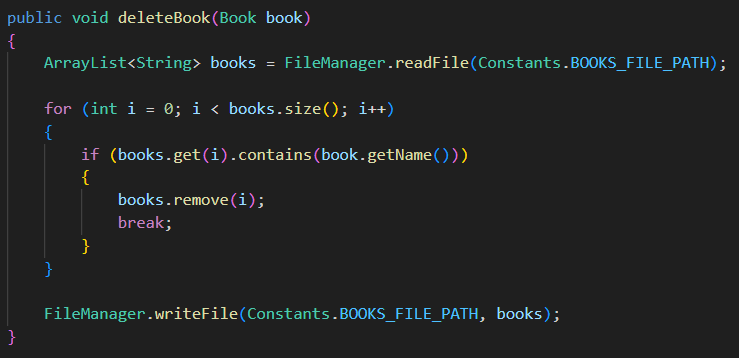
\includegraphics[width=\textwidth]{Media/deleteBook.png}
        \caption{deleteBook Implementation}
    \end{figure}
\end{itemize}

\newpage
\section*{Reader Functions}
New users can register as readers. Once the user fills in the required data, pressing Register will call the 
\texttt{register(String email, String username, String password, String phone\-Number, String address, String payment\-Method)} method.
\begin{figure}[H]
    \centering
    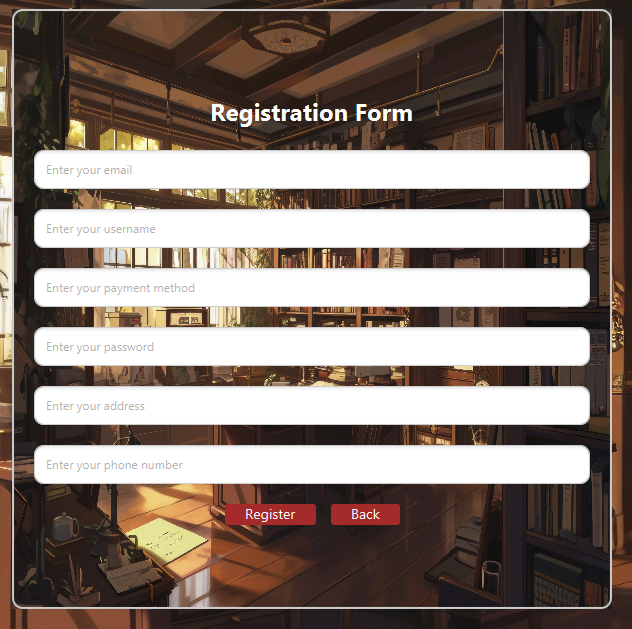
\includegraphics[width=0.6\textwidth]{Media/Register Form.png}
    \caption{Registration Form}
\end{figure}

\begin{figure}[H]
    \centering
    \makebox[\textwidth][c]{%
        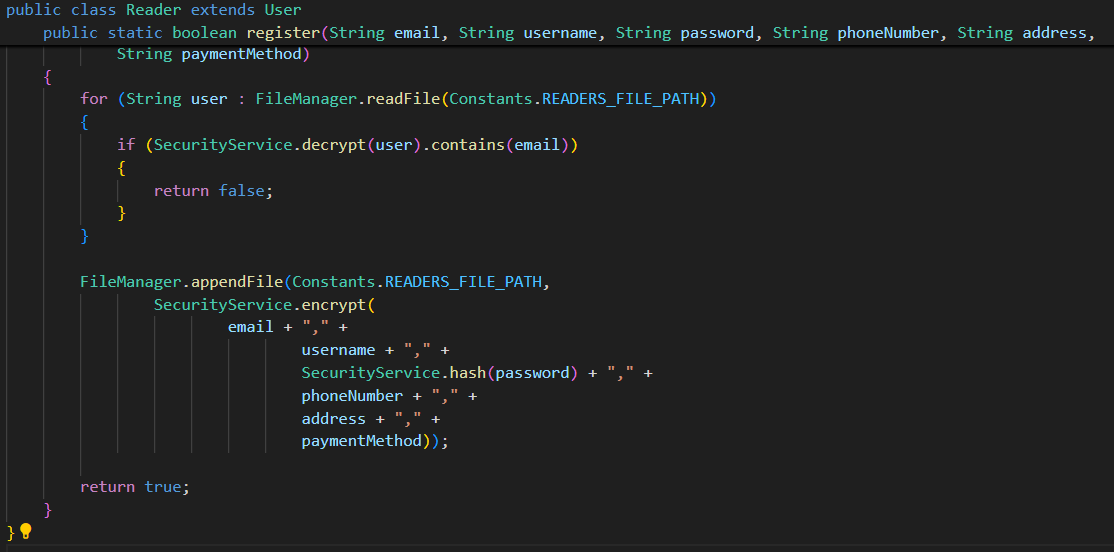
\includegraphics[width=\textwidth]{Media/register.png}
    }
    \caption{register Implementation}
\end{figure}

\newpage
\begin{figure}[H]
    \centering
    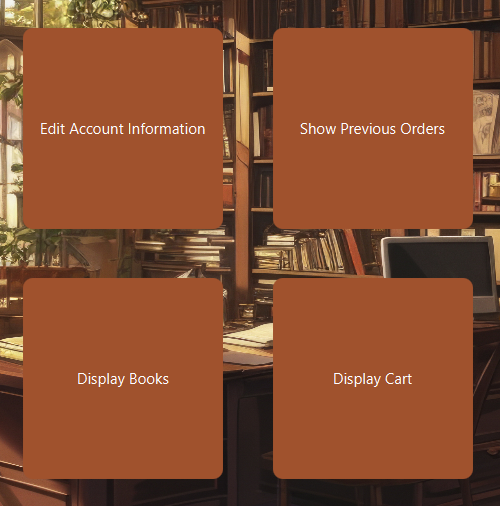
\includegraphics[width=0.9\textwidth]{Media/Reader Menu.png}
    \caption{Reader Menu}
\end{figure}
\newpage
\begin{itemize}

    \item \textbf{Edit Account Information:} The reader can edit his account information using the Edit Account Information page. Once the reader has modified his data, pressing yes will call the \texttt{update\-Reader\-Information()} method, which will update the user's data in the book store's database.
    \begin{figure}[H]
        \centering
        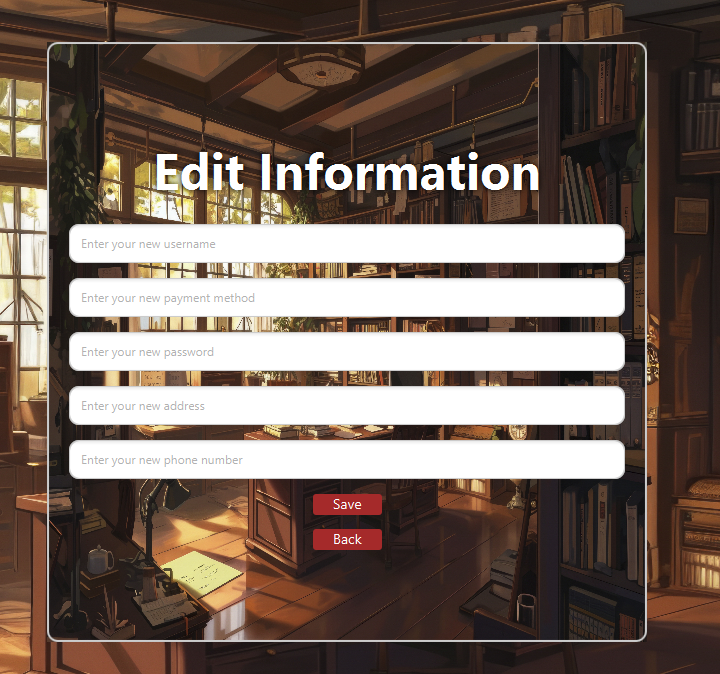
\includegraphics[width=0.7\textwidth]{Media/Edit Information.png}
        \caption{Edit Information Page}
    \end{figure}
    \begin{figure}[H]
        \centering
        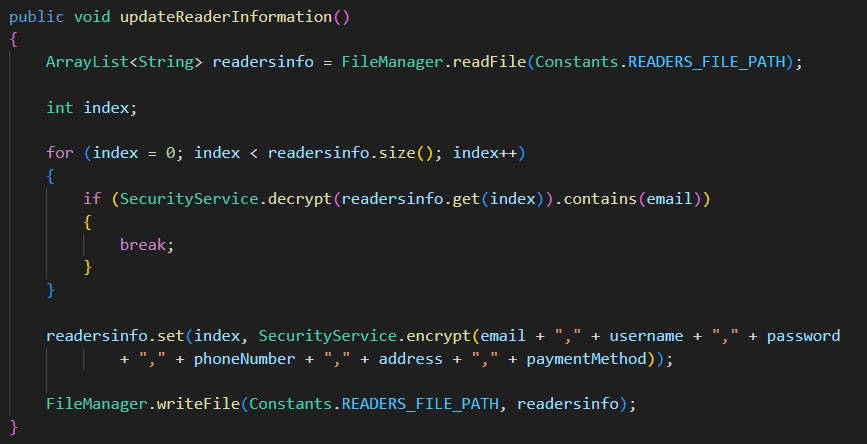
\includegraphics[width=0.85\textwidth]{Media/updateReaderInformation.png}
        \caption{updateReaderInformation Implementation}
    \end{figure}

    \item \textbf{Show Previous Orders:} The reader can view all his previous orders on this page.
    \begin{figure}[H]
        \centering
        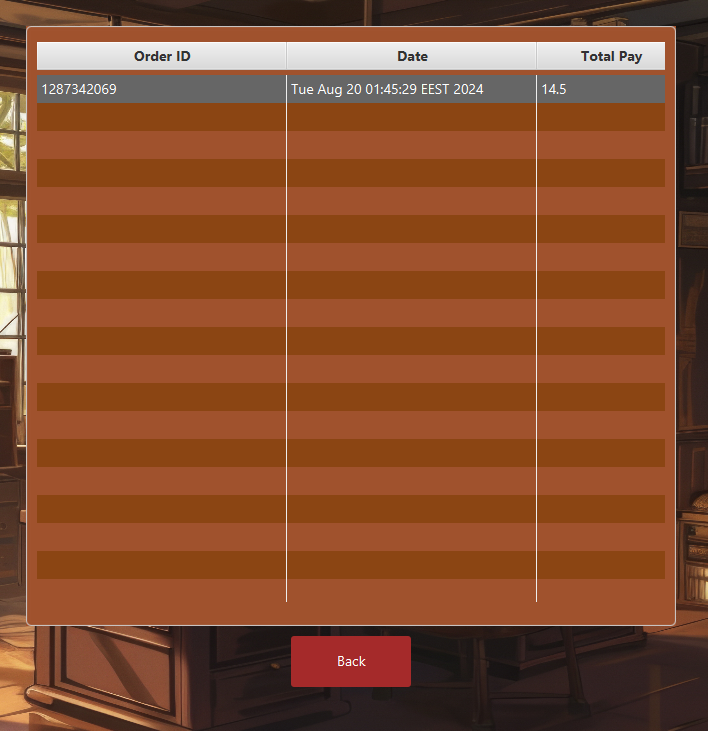
\includegraphics[width=0.6\textwidth]{Media/Show Previous Orders.png}
        \caption{Show Previous Orders Page}
    \end{figure}
    
    \begin{figure}[H]
    \centering
    \makebox[\textwidth][c]{%
        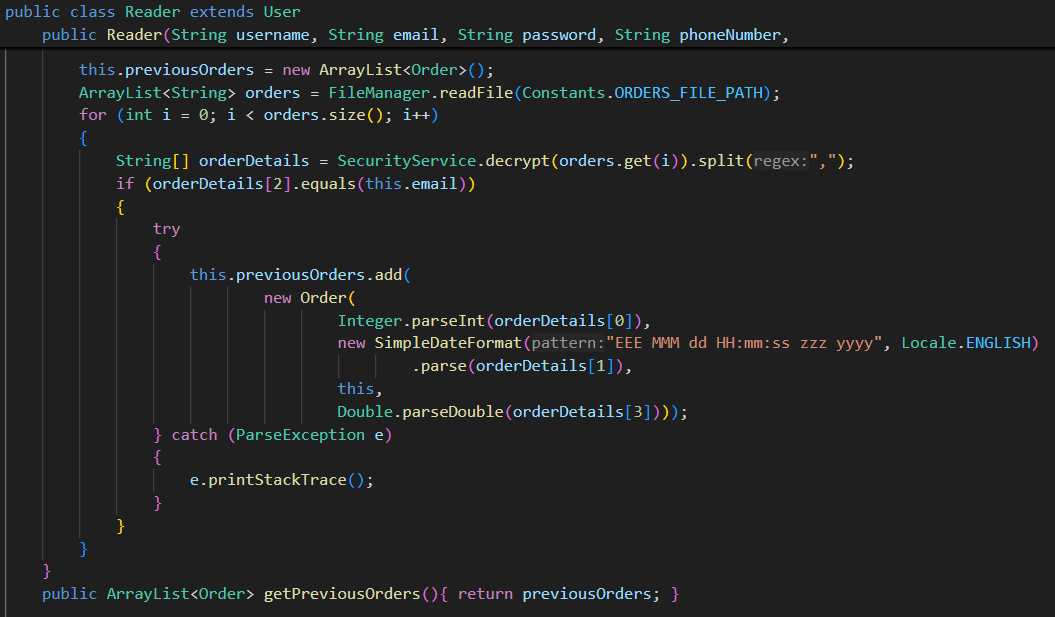
\includegraphics[width=\textwidth]{Media/previousOrders.png}
    }
        \caption{Initialization of the previousOrders ArrayList}
\end{figure}
\newpage
    \item \textbf{Display Books:} The reader can view all books *with stock more than 0* and can search for a specific book. The reader can select a book and add it to the cart.
    \begin{figure}[H]
        \centering
        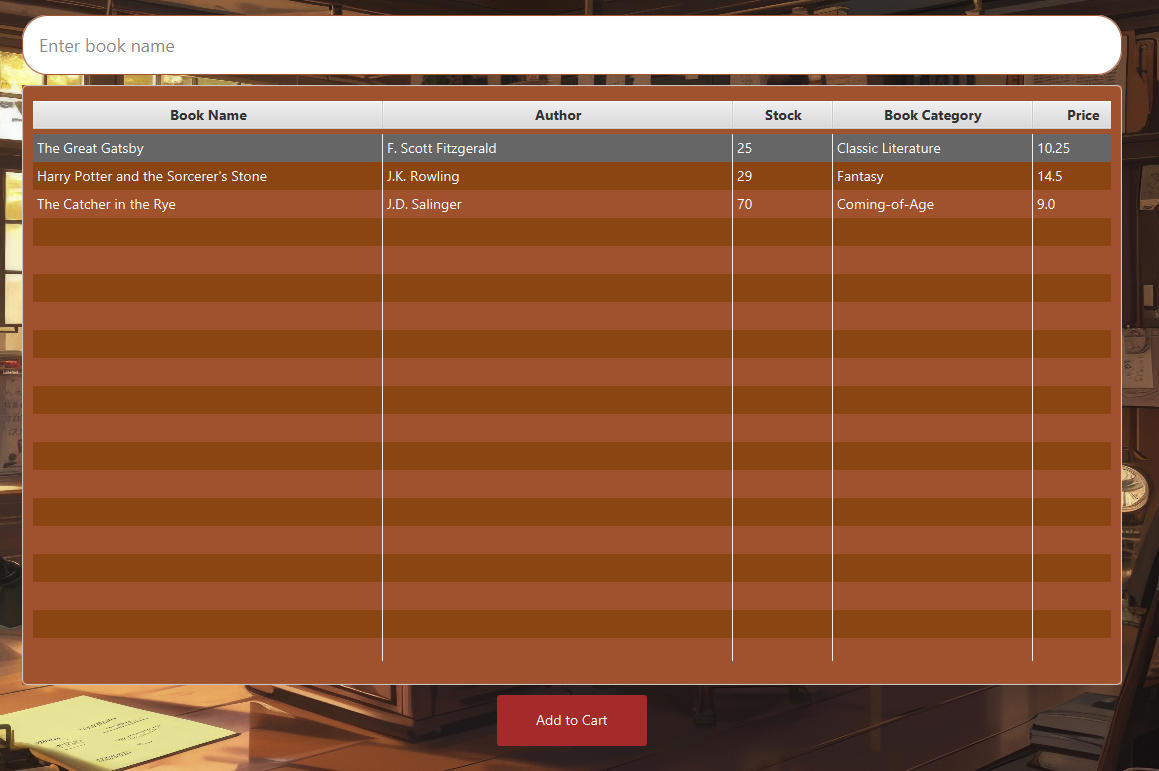
\includegraphics[width=\textwidth]{Media/Display Books.png}
        \caption{Display Books Page}
    \end{figure}
    Adding a book to the cart with the Add to Cart button will call the 
    \texttt{add\-To\-Cart(Book book)} method.
    \begin{figure}[H]
        \centering
        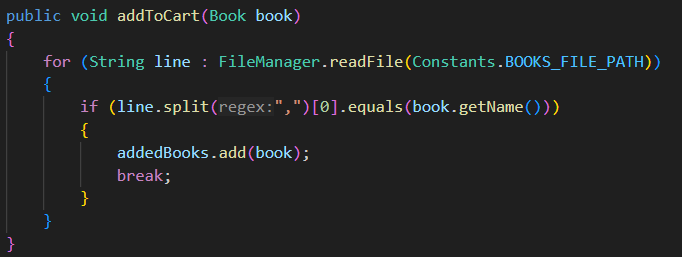
\includegraphics[width=0.85\textwidth]{Media/addToCart.png}
        \caption{addToCart Implementation}
    \end{figure}
\newpage
    \item \textbf{Display Cart:} The reader can view the books currently in his shopping cart on this page.
    \begin{figure}[H]
        \centering
        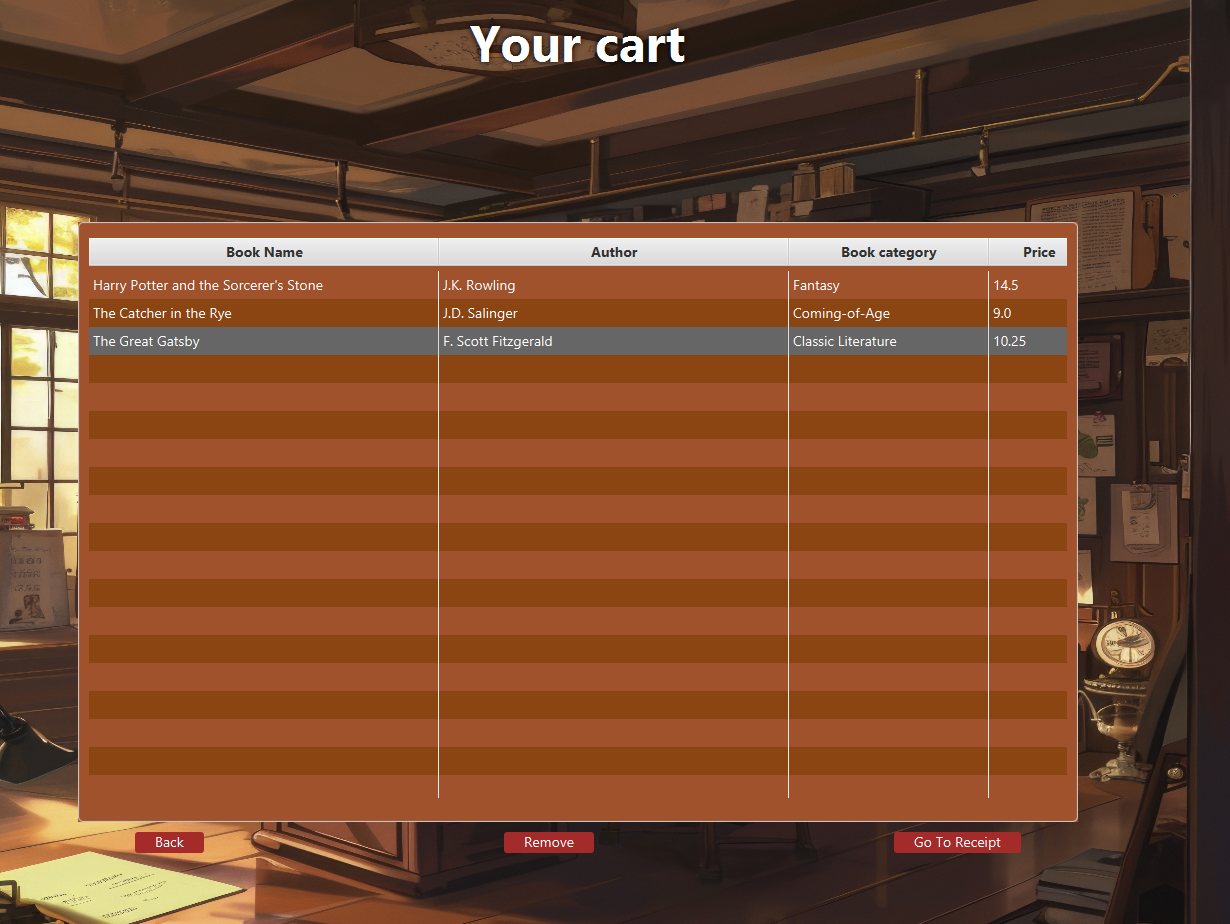
\includegraphics[width=\textwidth]{Media/Your Cart.png}
        \caption{Your Cart Page}
    \end{figure}

    The reader can also remove books from the cart, which will call the 
    \texttt{remove\-From\-Cart(Book bookToRemove)} method.

            \begin{figure}[H]
    \centering
    \makebox[\textwidth][c]{%
        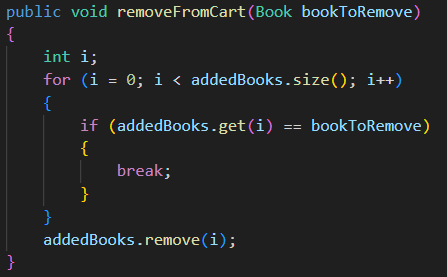
\includegraphics[width=0.65\textwidth]{Media/removeFromCart.png}
    }
        \caption{removeFromCart Implementation}
\end{figure}

    
\newpage
    \item \textbf{Go To Receipt:} In the receipt page, the user can use the Pay button, which will call the 
    \texttt{generate\-Order(ArrayList<Book> books)} method.
    
        \begin{figure}[H]
    \centering
    \makebox[\textwidth][c]{%
        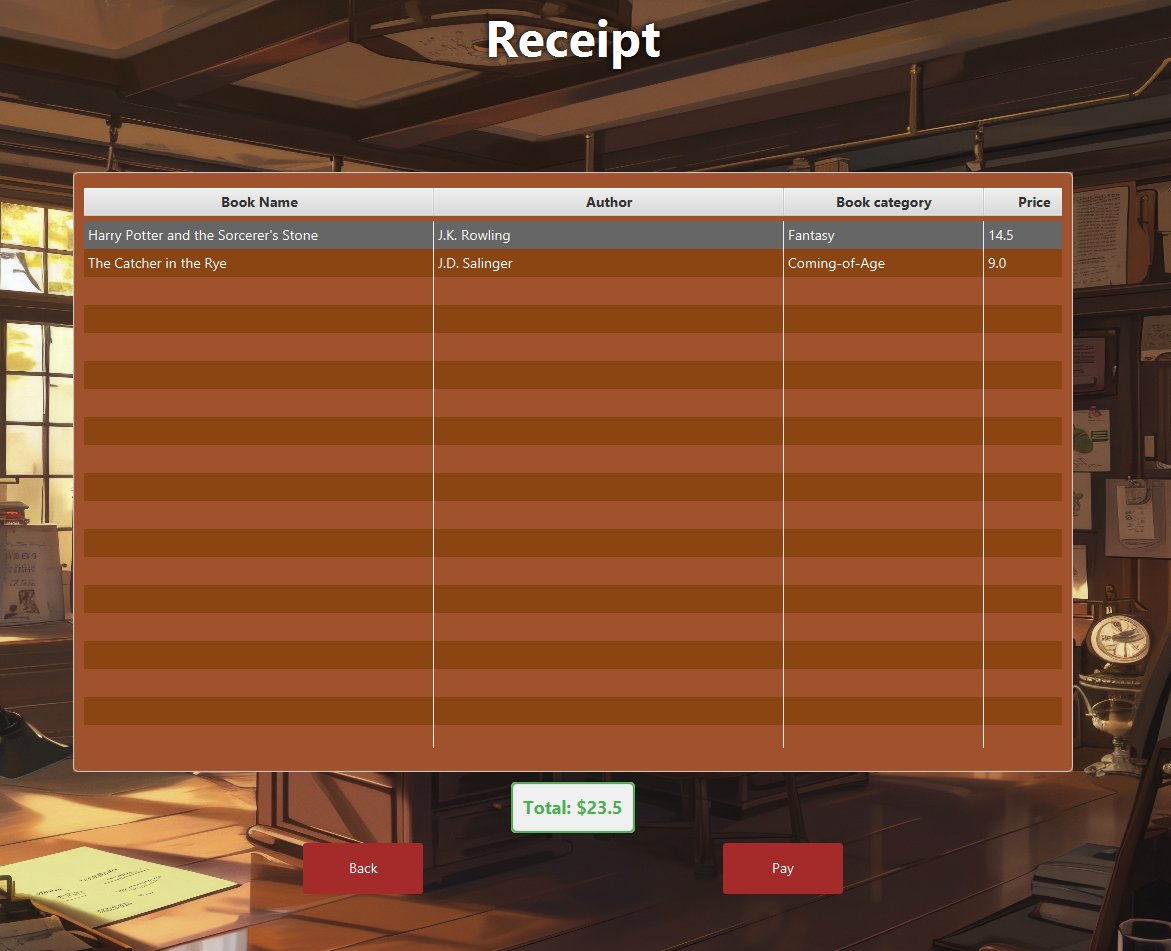
\includegraphics[width=\textwidth]{Media/Receipt.png}
    }
        \caption{Receipt page}
\end{figure}
    
        \begin{figure}[H]
    \centering
    \makebox[\textwidth][c]{%
        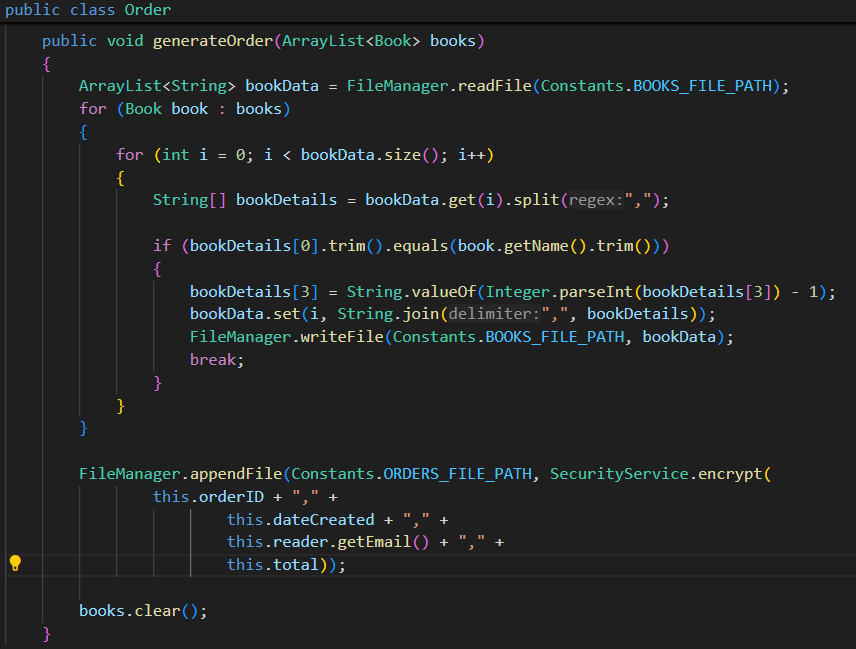
\includegraphics[width=\textwidth]{Media/generateOrder.png}
    }
        \caption{generateOrder Implementation}
\end{figure}

\end{itemize}

\end{document}
